\section{Workflow}
Here, we elaborate on the workflow for analyzing the \textit{GraphRAG} process.
\label{section 4}
\subsection{Overview}

\begin{figure}[ht]
  \centering
  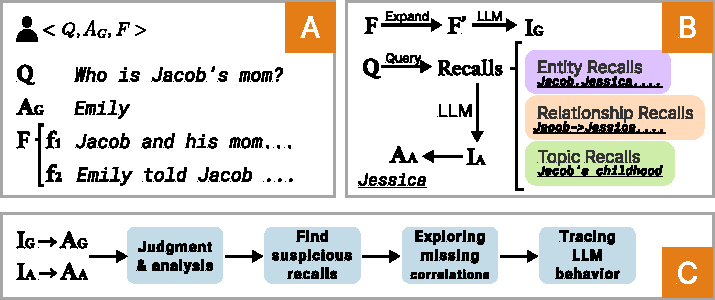
\includegraphics[width=\linewidth]{figs/Workflow2.pdf}
  \caption{Overview of the workflow: The user first prepares a testing pair for evaluation (A). Subsequently, two recall-inference-answer chains are constructed for comparison, corresponding to the ground truth answer and actual answer respectively (B). Finally, users conduct a step-by-step analysis of the issue through a linear exploration process (C).}
  \label{fig:overview}
  \vspace{-10pt}
\end{figure}

To assist users in exploring graph construction issues, we divide the entire methodological process into two stages:

\textbf{Identifying Suspicious Retrievals:} Users conduct a question-and-answer evaluation using test data to preliminarily identify contradictions between actual answers and the ground truth. By analyzing the inference paths of both the actual answers and the ground truth, users can pinpoint problematic inference steps and identify suspicious recalls, understanding what the issues are and where they occur.

\textbf{Analyzing Suspicious Retrievals:} Starting with the identified suspicious recalls, users conduct either local or global analyses based on the type of recall. They trace reference chains to investigate the behavior of LLMs, uncover issues in graph construction, and provide evidence for optimizing graph quality, thereby understanding why the issues occur and how to address them.

\subsection{Stage 1: Identifying Suspicious Retrievals}

The GraphRAG system utilizes an initial document collection $D$ ($d_i \in D$) to construct a graph $\mathcal{G}$. During the testing phase, users query the constructed graph with test pairs $<Q, A_G, F>$ to retrieve actual answers $A_A$, where $Q$ is the question, $A_G$ is the Ground Truth Answer and $F$ is the set of evidence facts (Fig~\ref{fig:overview}A).
We evaluate both the correctness of the generated answers and their corresponding inference steps, guiding users to explore the unexpected results.
For \textbf{answer evaluation}, we employ an LLM to judge the answer $A_A$ as \textit{correct} or \textit{wrong} based on the Ground Truth $A_G$.
For \textbf{assessing inference steps}, we develop an LLM-assisted analysis framework \cite{wang2023vis+} to reconstruct the inference process for generated answers and ground truth and compare them to identify suspicious retrieval recalls (Fig~\ref{fig:overview}B).
We describe the details of the analysis framework as follows.

\subsubsection{Inferences Process Construction}

We construct the inference process as a \textit{Question-Recalls-Inferring-Answer} pipeline to facilitate comparative analysis.

\textbf{Actual Answer Inferences $I_A$.} When users submit a query, the GraphRAG system first retrieves a series of recalls. These are processed by the LLM to generate detailed inference steps ($I_{A_i} \in I_A$), each step indicating the recalls it relies on.

\textbf{Ground Truth Inferences $I_G$.} For the Ground Truth, each fact $F_i \in F$ from the test pair is contextually expanded to $F'_i \in F'$ to facilitate inferring, as the original facts may lack sufficient context. The expanded context test pair $<Q, A_G, F'>$ is then submitted to the LLM for reverse inferring, resulting in detailed inference steps $I_G$ based on $Q$ and $F'$, with each step specifying the facts utilized.

Each fact $F_i$ corresponds to several original document chunks. Entities and relationships related to these chunks are extracted to form a fact subgraph $\mathcal{G}_{F_i}$. For each inference step $I_{G_i}$, the relevant fact subgraphs are merged and filtered by the LLM to select entities and relationships pertinent to that step, forming the inference subgraph $\mathcal{G}_{G_i}$.

Finally, the entities and relationships in the inference subgraph $\mathcal{G}_{G_i}$ are used as recalls for each inference step $I_{G_i}$.

\subsubsection{Suspicious Recall Identification}

Based on the inference steps of Ground Truth $I_G$ and the Actual Answer $I_A$, users perform a comparative analysis to pinpoint problematic inference steps and identify the corresponding recalls for discrepancies. We flag two types of recalls as suspicious: \textbf{Missing Recalls}, which are essential to critical inference steps in the correct answer but absent from the actual inference steps, necessitating analysis to determine why they were not retrieved or used; and \textbf{Unexpected Recalls}, which do not belong to the critical inference steps in the correct answer but are erroneously included in the actual inference steps, requiring investigation to understand why they were mistakenly retrieved or utilized.

\subsection{Stage 2: Analyzing Suspicious Retrievals}

In the previous phase, users identified suspicious retrievals by analyzing problematic inference steps. To further investigate the causes of these issues in the GraphRAG system, users must dive into the internal structure of the system to explore the relationships between entities, relationships, and topic reports. This involves tracing the construction and retrieval processes to uncover the behavior of the LLM, continuing until the root cause of the issue is clarified (Fig~\ref{fig:overview}C).

\subsubsection{Exploring Missing Correlations}

The exploration of missing correlations is categorized into local and global investigations based on recall types, aiming to identify and address missing correlation information. \textbf{Local exploration} focuses on entity and relationship recalls, requiring users to examine their relationships with other entities and relationships. Specifically, these relationships may include connections with entities mentioned in the question, entities referenced in the correct answer, or entities involved in critical inference steps.

For \textbf{global exploration}, which centers on topic report recalls, users investigate their relationships with other reports. These relationships may include connections to topic reports that reference entities mentioned in the question or entities included in the correct answer. Through this structured approach, users can systematically trace missing correlations and enhance their understanding of the underlying retrieval process.

\subsubsection{Tracing LLM Behavior}

Once a recall with missing correlation information is identified, further tracing of the LLM's behavior is necessary to pinpoint where in the construction process this information was lost.

In the construction and retrieval stages of the GraphRAG system, each stage involves references to preceding content, with the LLM playing a crucial role. This forms the foundation for tracing and analyzing the behavior of the LLMs:

\begin{itemize}
    \item \textbf{Extract}: The LLM extracts multiple entities and relationships from chunks.
    \item \textbf{Merge}: The LLM consolidates same-named entities and relationships, referencing entity-chunks or relationship-chunks.
    \item \textbf{Summarize}: The LLM summarizes entities and relationships within a topic subgraph to create a topic report.
    \item \textbf{Infer}: The LLM uses query retrievals for reasoning, referencing inference step-entities and relationships.
\end{itemize}

To identify issues in different types of suspicious recalls, users undertake distinct tracing analyses. For entity and relationship recalls, the process involves analyzing the merging behavior and subsequently examining the extraction behavior. In the case of topic report recalls, a comprehensive investigation is conducted, focusing on the summarization, merging, and extraction behaviors.